\documentclass{article}
\usepackage[letterpaper, margin=1.25in]{geometry}
\usepackage{graphicx}
\usepackage[colorlinks=false]{hyperref}
\usepackage{capt-of}
\usepackage{listings}

\begin{document}

\title{Using 10Base--T Ethernet\\for Underwater Optic Communication}
\author{UC the Fish}

\maketitle

\section{Introduction}

One functional requirement for UC the Fish was modular optic communication,
or the communication system should be easy to integrate with devices that need to
communicate; a plug--and--play solution.

Nearly every modern computer has at least \mbox{10Base--T Ethernet} and
\mbox{USB 2.0} connectivity, so any ``modular'' communication attachment
should use one of these protocols--at least at its endpoints.
We chose to \mbox{10Base--T Ethernet}, not just at the interfaces but to
send the Ethernet signal itself through water in the form of intensity
of blue light.
This allowed us to focus on building blue light transmit and receive
hardware instead of attempting to develop light transmit/receive hardware
\textit{and} a modulation protocol + logic giving it USB endpoints.

Ethernet allows multiple stations to share a single medium,
which is appropriate for water because light spreads in every direction
and data cannot be multiplexed over different wavelength channels. 
It includes hardware support for cyclic redundancy bit checking,
up to 16 retransmission attempts in the case of bit errors or disruption
of the medium, and at \mbox{10 MHz}, Ethernet is fast enough 
for live streaming video.

Unlike USB, a temporary disruption in the data link does not require
renegotiation time and application level link management.
Software applications can use the operating system to handle TCP protocol
when data integrity and delivery acknowledgement are necessary, instead
of writing custom code to ensure control commands reach the sub intact.

\section{Getting the Standard}

IEEE Std 802.3 is the standard for Ethernet communication.
It is freely available online but is so large it is split into multiple
sections.
The first section (only 555 pages!) is available at
\url{https://standards.ieee.org/getieee802/download/802.3-2012\_section1.pdf}.

\section[title]{Ethernet 101 \footnote{Or in other words, an Ethernet Preamble. Hehe.}}

Ethernet is a time domain communication protocol for connecting any number of
machines via a single, shared medium.
Each \textit{station} is given a unique address when it is manufactured and
data is sent serially--1 bit at a time--in \textit{packets} between
stations.

\begin{center}
	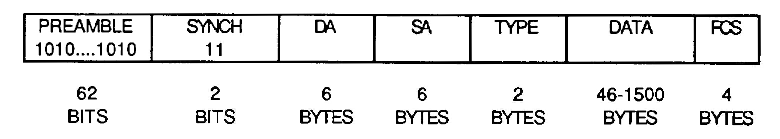
\includegraphics[width=0.75\textwidth]{ethernet-packet.pdf}
	\captionof{figure}{Format of an Ethernet Packet.}
	\label{packet-format}
\end{center}

Time sharing of the medium is done by all stations following
\textit{Carrier Sense Multiple Access with Collision Detection}
(CSMA/CD) protocol.
Only one station may transmit at a time and all stations constantly
monitor the line, looking for packets addressed to them and seeing when
the line is open for transmission (CSMA).
After completion of a packet, all stations wait an
\textit{interpacket gap} before attempting to transmit a packet of their own.
If two stations transmit at the same time, both detect a collision
and backoff for a period of time (/CD).
A pseudo random exponential backoff algorithm is used to make repeat
collisions unlikely and retransmission is attempted up to 16 times
below the level of the operating system.

\section{More Details from the Standard}

\begin{center}
	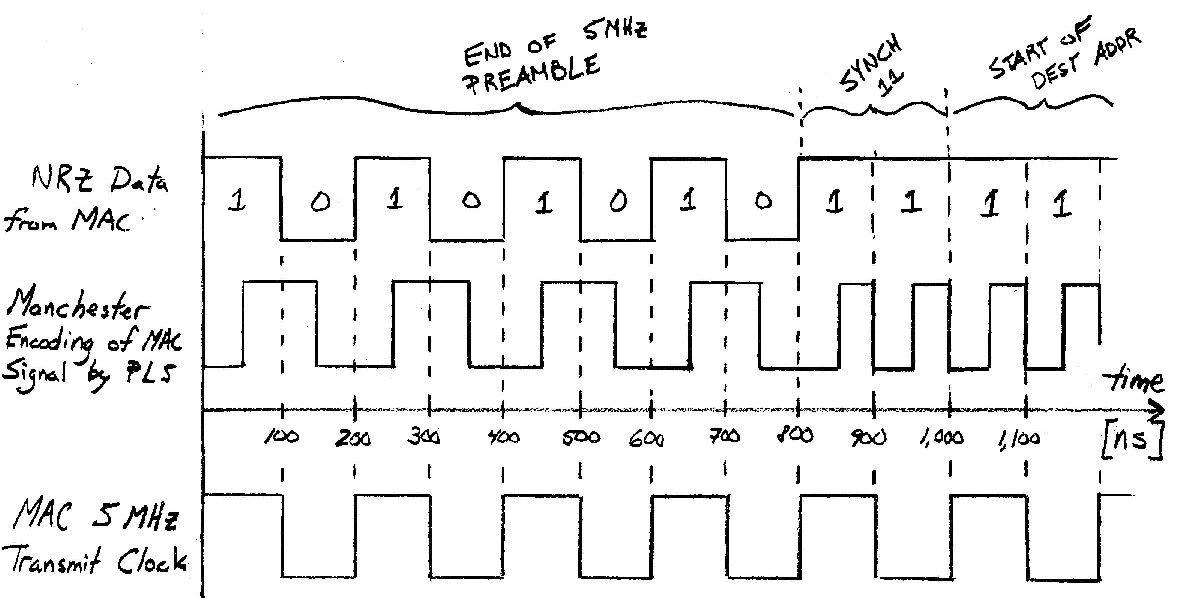
\includegraphics[width=0.75\textwidth]{timing-diagram.pdf}
	\captionof{figure}{Non--return to Zero and Manchester Encoding.}
	\label{timing-diagram}
\end{center}



\section{Influence on Transmitter/Receiver Design}

\begin{enumerate}
\item The first component in the light transmitter input
and last component of the receiver output should be a 1:1, Ethernet approved
transformer and standard RJ45 connector.
\item The input impedance of light transmitter must be $100\,\Omega$.
\item The bandwidth of both light transmitter and receiver must exceed $10\,MHz$
by several harmonics, and
\item their phase shift between $5\,MHz$ and $10\,MHz$ should be negligible.
\item The magnitude response of light transmitter + receiver in series,
to a $100\,ns$, $585\,mV$ step input, should be $\geq585\,mV$ when loaded by $100\,\Omega$.
\end{enumerate}

\section{Limitations for Underwater Communication}

There are two limitations associated with sending 10Base--T Ethernet signals,
unmodified, through water by modulating light intensity.
Both are related to the separation of transmit and receive pairs
in 10Base--T, and how stations detect collisions.

First, is the isolation of transmit and receive signals in twisted--pair media.
The 10Base--T Ethernet hardware on modern computers expect to operate in full
duplex mode, that is when they still listen on the receive line for when
other stations own the network, but when they transmit they expect silence
on the receive pair--they do not expect to hear their own signal.
If the station hears anything on the receive line when it is transmitting,
it interprets it as a jam signal from a router and stops transmitting immediately.

This is a limitation in sending Ethernet as light: there will be some
level of reflected light due to the optical interface and from particles in the water.
If the receiver circuit is built to have a fixed gain, then it must be below
the threshold at which it would jam itself.

To determine at what distance and signal magnitude this might occur,
tested the current response of the photodiode to the blue LED with 20 mA current
in water at different distances.
A 5 inch acrylic security camera dome was used and the test was performed in
tap water.
The results, shown in figure \ref{crossover-point} suggested that the overall gain
should be less than
\begin{equation}
|Z_{gain}| \leq \frac{V_{\textrm{threshold}}}{I_{reflected}}=\frac{585\,mV}{26\,nA}=22.5*10^{6}\,\Omega
\end{equation}
and that the maximum distance 10Base--T Ethernet could be transmitted with purely analog transmit/receive
circuits is about 25 centimeters.

\begin{center}
	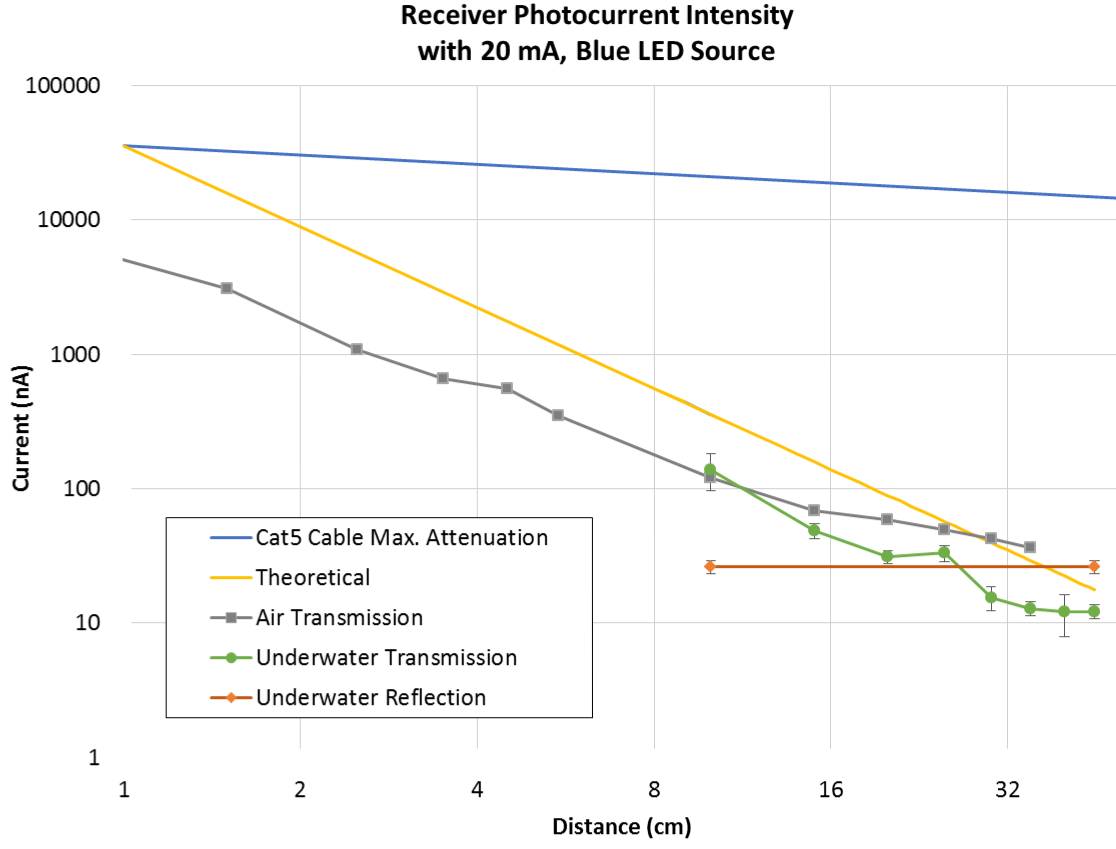
\includegraphics[width=0.8\textwidth]{crossover-point.pdf}
	\captionof{figure}{Crossover Point: the distance at which reflected light from \mbox{station A's} own transmitter is more intense than
light arriving from far--away \mbox{station B's}. I.e. the distance at which water/light stop behaving like an Ethernet crossover cable.}
	\label{crossover-point}
\end{center}

The second limitation of 10Base--T Ethernet is due to the required \textit{link integrity test}
specified in the standard.
A station is not allowed to transmit unless it hears either incoming packets or
a special pulse from a router indicating no traffic but good connection.
This means that a one--way link cannot be tested; both directions must be complete
in order for either station to send out data.

This does not limit the final product, but it does make it more difficult to test
prototypes: two transmit and two receive circuits must be built and if
any one piece doesn't work, then neither computer will even try to broadcast data.
To help with this problem, UC the Fish built a special Ethernet cable with
one Tx--Rx pair connected and the other opened with Tx and Rx RJ45 plugs.
The cable can be used as shown in figure \ref{ethernet-test-setup}.

\begin{center}
	\includegraphics[width=1\textwidth]{ethernet-test-setup}
	\captionof{figure}{UC the Fish Test Setup, using custom crossover cable,
two Linux PCs, and test programs 
\texttt{broadcast\_packet.c} and \texttt{ethernet\_listen.c}.}
	\label{ethernet-test-setup}
\end{center}

\appendix

\pagebreak
\section{Ethernet Test Scripts}

\lstinputlisting{Makefile}

\pagebreak
\lstinputlisting{broadcast_packet.c}

\pagebreak
\lstinputlisting{ethernet_listen.c}

\end{document}
